\section{The t-test}
One way to test hypothesis about any single parameters in the population regression function is to make use of the t-test. 
A t-test is an inferential statistic determining whether or not the difference between two t statistics, e.g. the means of two groups, is significant. 
Recall that OLS produces unbiased estimates. 

Throughout this section, given $j\in\{ 1, \ldots, k\}$, let $d_j=(X^TX)^{-1}_{jj}$ denote the $j2$'th diagonal element of $(X^TX)^{-1}$, let $\hat{\beta}_j(\textbf{y})$ denote the j'th coordinate of the MLE $\hat{\beta}(\textbf{y})$ and $\hat{\sigma}^2(\textbf{y})$ denote the usual estimate for $\sigma^2$.

In order to construct hypothesis test, the following result is needed.

\begin{theorem} [Test of Individual Parameters] \label{th:t_distribution}
Let $\beta_{0j}$ be given and consider the hypothesis $\mathcal{H}_0=\beta_{0j}$. Under the assumptions \ref{as:linear_in_the_parameters}, \ref{as:no_perfect_collinearity}, \ref{as:zero_conditional_mean}, \ref{as:homoskedasticity_and_no_serial_correlation} and \ref{as:normality_of_errors} the t-test for $\mathcal{H}_0$ is given by
\begin{align}
   t_j(\textbf{y};\beta_{0j}) = \frac{\hat{\beta}_j - \beta_{0j}}{\sqrt{d_j\sigma^2(\textbf{y})}}\sim t_{n-k-1} = t_{df}, \quad for \ j=1,\ldots,k
\end{align}
where $k+1$ is the number of unknown parameters in the population model \eqref{eq:multiple_linear_regression}, $n-k-1$ is the degrees of freedom (df) and large values of $|t_j(\textbf{y};\beta_{0j})|$ are critical for $\mathcal{H}_0$.

And the p-value is
\begin{align}
    p(\textbf{y},\beta_{0j})=P(|t_j(\textbf{Y};\beta_{0j})|\leq |t_j(\textbf{y};\beta_{0j})|).
\end{align}
Futhermore, for $0<a<1$, using the t-test at level $a$, the limits of a ($1-a$)-confidence interval for $\beta_j$ is
\begin{align}
    \hat{\beta}_{j}(\textbf{y}) \pm t_{1-a/2}(n-k-1)\sqrt{d_j\sigma^2(\textbf{y})}
\end{align}
which corresponds to those cases where we accept the hypothesis that $\beta_j$ takes a specific value.
\end{theorem}
\begin{proof}
Recall due to the assumptions \ref{as:linear_in_the_parameters}, \ref{as:no_perfect_collinearity}, \ref{as:zero_conditional_mean}, \ref{as:homoskedasticity_and_no_serial_correlation} and \ref{as:normality_of_errors}

\begin{align} \label{eq:th_t_test}
    \hat{\beta}(\textbf{Y}) \sim N_k(\beta,\sigma^2(X^TX)^{-1})
\end{align}
and thus
\begin{align*}
    (\hat{\beta}(\textbf{Y})-\beta_j)/\sqrt{d_j\sigma^2(\textbf{Y})} \sim N(0,d_j \sigma^2) \quad \text{and} \quad \sigma^2(\textbf{Y}) \sim \sigma^2\chi (n-k)/(n-k)
\end{align*}
are independent. Therefore
\begin{align*}
    t_j(\textbf{Y};\beta_j)=\frac{(\hat{\beta}(\textbf{Y})-\beta_j)/\sqrt{d_j\sigma^2(\textbf{Y})}}{\sigma^2(\textbf{Y})/\sigma^2} \sim t(n-k)
\end{align*}
and the first part of the theorem composed of \eqref{eq:th_t_test} is verified, and second part follows immediately. 
\end{proof}

The pdf of the t distribution has a shape that is similar to the standard normal distribution. Except that it is more spread out in the tails and thus has larger areas in the tails. In figure \ref{fig:t_distribution} the pdf of the t distribution is plotted for various degrees of freedom. 

\begin{figure}[h]
    \centering
    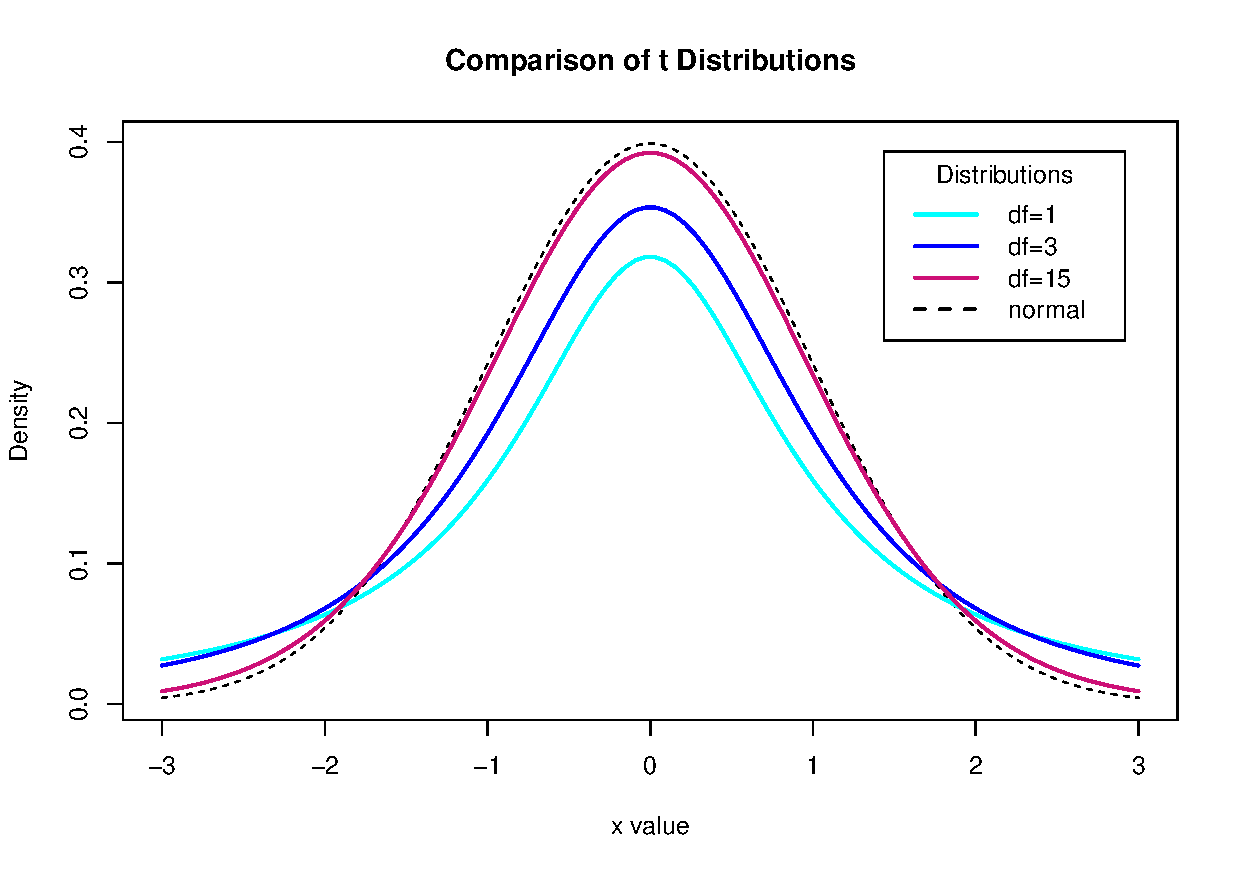
\includegraphics[width = 0.9\textwidth]{figures/t_distribution.pdf}
    \caption{The t distribution for various DF compared to the standard normal distribution.}
    \label{fig:t_distribution}
\end{figure}

Clearly, as the degrees of freedom increases, the t distribution approaches the standard normal distribution.

The primary interest is testing the null hypothesis
\begin{align} \label{eq:t_test_h0}
    \mathcal{H}_0=\beta_j=0, \quad for \ j=1,\ldots,k.
\end{align}
Since after controlling for all other independent variables than $x_j$, $\beta_j$ measures the partial effect of $x_j$ on the expected value of $y$. 
Thus \eqref{eq:t_test_h0} means that, after $x_1,x_2, \ldots, x_{j-1}, x_{j+1}, \ldots, x_k$ have been accounted for, $x_j$ has no effect on the expected value for $y$ since $\beta_j=0$. 
For $x_j$ having a partial effect on the expected value of $y$, the value of $\beta_j$ has to be anything other than zero.

In practice, $\hat{\beta}$ will not be zero, whether or not $\mathcal{H}_0$ is true. Therefore the question is rather how to determine how far $\hat{\beta}_j$ is from zero. The further the sample value of $\hat{\beta}_j$ is from zero, the bigger is the evidence against $\mathcal{H}_0$. However, on the other hand the larger the sampling error is of $\hat{\beta}_j$, the smaller is the evidence against $\mathcal{H}_0$. Thus $t_{\hat{\beta}_j}$ is a ratio of how many estimated standard deviations $\hat{\beta}_j$ is away from zero. In general the larger value of $t_{\hat{\beta}_j}$, the larger the evidence against $\mathcal{H}_0$. The precise rule for rejecting $\mathcal{H}_0$ depends on the alternative hypothesis and the chosen significance level.

\subsection{Prediction}

Suppose an observed realization of $\textbf{Y}=\textbf{y}$, however, the extra random variable 

SKRIVES UD FRA JAKOBS NOTER!!!!!!

\subsection{Testing against Two-Tailed Alternatives}

ARGUMENTER FOR TWO TAILED IFT TEST AF OLS ESTIMATER

EKSEMPEL SKRIVES IND HER (ER LAVET)

As the alternative hypothesis a one-sided alternative of the form
\begin{align}\label{eq:onesided_alt}
    \mathcal{H}_1:\beta_j>0 , \quad for \ j=1,\ldots,k
\end{align}

is considered and thus

\begin{align}\label{eq:onesided_h0}
    \mathcal{H}_0=\beta_j \leq 0 , \quad for \ j=1,\ldots,k.
\end{align}





%\textit{\section{likelihood ratio tests}

%\begin{theorem}[theorem title]
%the likelihood ratio test statistic for testing the hypothesis
%\begin{align}
%\mathcal{h}_0:\boldsymbol{\mu} \in \omega_0
%\end{align}
%against the alternative hypothesis
%\begin{align}
%\mathcal{h}_1:\boldsymbol{\mu} \in \omega_1 \backslash \omega_0
%\end{align}
%is a monotone function of 
%\begin{align}
%f(\boldsymbol{y})=\frac{d(p_1(\boldsymbol{y});p_0(\boldsymbol{y}))/(m_1-m_0)}{d(\boldsymbol{y};p_1(\boldsymbol{y}))/(n-m_1)}
%\end{align}
%where $p_1(\boldsymbol{y})$ and $p_0(\boldsymbol{y})$ are projections of $\boldsymbol{y}$ on $\omega_1$ and its subset $\omega_0$, respectively.
%under the assumption of $\mathcal{h}_0$ 
%\begin{align}
%f = f(m_1-m_0,n-m_1)
%\end{align}
%\end{theorem}}



\begin{definition} [The (1-a)-confidence Region]
\label{def:confidence_region}
Suppose that for a given number $a \in (0,1)$ and for each $\textbf{y} \in \mathcal{Y}$, we have specified a subset $A(\textbf{y})$ of the parameter space $\Theta^k$, such that
\begin{align*}
    P_{\boldsymbol{\beta}} (\boldsymbol{\beta} \in A(\textbf{Y})) = 1 - a, \quad \forall \boldsymbol{\beta} \in \Theta^k
\end{align*}
Then we call $A(y)$ a $(1-a)$-confidence region for $\boldsymbol{\beta}$.
\end{definition}

If the parameter is one-dimensional $(k=1)$ and the observations, $y$ are normally distributed, then the confidence region become the interval

\begin{align*}
    \left[ 
    \hat{\beta}(\textbf{y}) + \Phi_{a/2} \sqrt{D(\hat{\beta}(\textbf{y})} , \hat{\beta}(\textbf{y}) + \Phi_{1 - a/2} \sqrt{D(\hat{\beta}(\textbf{y})}
    \right]
\end{align*}

for $0 < a \leq 0.5$. 


\begin{example}
Consider again the situation from example \ref{ex:model1}. By theorem \ref{th:distribution_ml_estimator} the asymptotic distribution of the ML estimator is given by
\begin{align*}
    \hat{\alpha} \rightarrow^\mathcal{D} N\left( \alpha, \boldsymbol{i}(\hat{\alpha})^{-1} \right)
\end{align*}

Since $\alpha$ is one-dimensional, $k=1$, and for $0\leq a \leq 0.5$ we have the approximate $(1-a)$-confidence interval
\begin{align*}
\left[ \hat{\alpha}(\mathbf{y}) + \Phi_{a/2} \sqrt{D\left( \hat{\alpha}\left(\mathbf{y}\right)\right)}, \hat{\alpha}(\mathbf{y}) + \Phi_{1 - a/2} \sqrt{D\left( \hat{\alpha}\left(\mathbf{y}\right)\right)} \right],
\end{align*}
where $D\left(\hat{\alpha}(\mathbf{y})\right) = j\left(\hat{\alpha}(\mathbf{y})\right)^{-1}$.
For $a=0.05$ we have the approximate $95\%$-confidence interval for $\alpha$:
\begin{align*}
\left[ \bar{y} - \frac{1.96}{\sqrt{n}}, \bar{y} + \frac{1.96}{\sqrt{n}} \right]    
\end{align*}
\end{example}


\section{F Test}

Suppose we want to test if a model has redundant explanatory variables.
In terms of hypothesis testing this is the null hypothesis: A set of variables has no statistically significant effect on $y$, once another set of variables has been controlled for. 

Determining this will be done by analyzing the change in SSR, that is the difference in how well the models explain the data, and determining whether this change is significant. 
Suppose we have model 1 with $(k+1)$ variables 
\begin{align*}
    y = \beta_0 + \beta_1 x_1 + \cdots + \beta_k x_k + \varepsilon,
\end{align*}
this is known as the unrestricted model. The restricted model or model 0 lacks the $q$ variables, for which we want to check significance, that is
\begin{align*}
    y = \beta_0 + \beta_1 x_1 + \cdots + \beta_{k-q} x_{k-q} + \varepsilon.
\end{align*}
This means we want to test the hypothesis
\begin{align}
    \mathcal{H}_0: \beta_{k-q+1} = 0 \ldots \beta_k = 0.
\end{align}
These are referred to as the exclusion restrictions. 
This is done using the F statistic
\begin{align}\label{eq:F_test}
    F \equiv \frac{\| H_1 y - H_0 y \|^2/q}{\| y - H_1 y \|^2/(n-k-1)},
\end{align}
that is the relative increase in $SSR$, when going from model 0 to model 1. 
$\| y - H_0 y \|^2$ is the $SSR$ of model 0 and $\| y - H_1 y \|^2$ is that of model 1. 
$q$ is referred to as the numerator degrees of freedom, and $(n-k-1)$ is the denominator degrees of freedom. 

The change in SSR, when going from model 0 to model 1, is always an increase because the model has more parameters to explain the data. 
This is discussed further in theorem \ref{th:Likelihood_ratio_linear_models}.

We will therefore reject $\mathcal{H}_0$, when $F$ is sufficiently large, since this indicates that significantly more of the variation of the data has been explained by model 1, as compared to model 0.

As with the t statistic, there is no correct significance level, but $a = 5 \%$ is often used. 
The critical value for the significance level can be determined either by calculating one explicitly from the F distribution found below or finding it in a table. 

$\mathcal{H}_0$ is therefore rejected if the F statistic is greater than the critical value
\begin{align*}
    F>c.
\end{align*}
If this is the case, the explanatory variables $x_{k-q+1}, \ldots, x_k$ are said to be jointly statistically significant. Otherwise they are said to be jointly insignificant, which can justify removing them from the model. 

\begin{definition}[F Distribution]
    Let $X_1 \sim \chi_{k_1}^2$ and $X_2 \sim \chi_{k_2}^2$ be independent random variables. Then the random variable 
        \begin{align*}
            F = \frac{X_1/k_1}{X_2/k_2}
        \end{align*}
    has an F distribution with $(k_1, k_2)$ degrees of freedom, which is denoted as $F \sim F_{k_1, k_2}$.
\end{definition}

The likelihood ratio can compare the goodness of fit for 2 models, specifically one over the entire parameter space and one with a restriction imposed.
It would therefore be interesting to see what relation it has to the F-test.

\begin{theorem}[Likelihood Ratio For Linear Models]
\label{th:Likelihood_ratio_linear_models}
    The Likelihood ratio
    \begin{align*}
        \lambda(y) = \frac{sup \ L(\mu_0, \sigma_0^2; y)}{sup \ L(\mu_1, \sigma_1^2; y)}
    \end{align*}
    is a strictly decreasing function of $F(y)$ under $\mathcal{H}_0$, such that
    \begin{align*}
        F(Y) \sim F(q, n-k-1).
    \end{align*}
\end{theorem}

\begin{proof}
    Under $\mathcal{H}_1$: $\hat{\mu}_1 = H_1 y$ and $\hat{\sigma}_1^2 = \frac{\| y - H_1 y \|^2}{n}$, the log likelihood function is
    \begin{align*}
        l(\hat{\mu}_1, \hat{\sigma}_1^2; y) &= -\frac{n}{2} log(\hat{\sigma}_1^2) - \frac{1}{2 \hat{\sigma}_1^2} \| y - H_1 y \|^2 \\
        &= -\frac{n}{2} log(\hat{\sigma}_1^2) - \frac{n}{2},
    \end{align*}
    and similarly for $\mathcal{H}_0$. Therefore the likelihood ratio can be written as
    \begin{align*}
        \lambda(y) &= exp \left( l(\hat{\mu}_0, \hat{\sigma}_0^2; y) - l(\hat{\mu}_1, \hat{\sigma}_1^2; y) \right) \\
        &= exp \left( -\frac{n}{2} \Big( log(\hat{\sigma}_0^2) - log(\hat{\sigma}_1^2)\Big) \right) \\
        &= \left( \frac{\| y - H_1 y \|^2}{\| y - H_0 y \|^2} \right)^{\frac{n}{2}} \\
        &= \left( \frac{\| y - H_1 y \|^2}{\| y - H_1 \|^2 + \| H_1 y - H_0 y \|^2} \right)^{\frac{n}{2}} \\.
    \end{align*}
    The last equation holds because $y - H_1 y$ is orthogonal to $\Omega_1$ and $(H_1 y - H_0 y) \in \Omega_1$. Dividing by the numerator and using \eqref{eq:F_test}, the above equation becomes
    \begin{align*}
        \lambda(y) &= \left( \frac{1}{1 + \frac{\| H_1 y - H_0 y \|^2}{\| y - H_1 y \|^2}} \right)^{\frac{n}{2}} \\
        &= \left( \frac{1}{1 + \frac{q}{n-k-1}F(y)}  \right)^{\frac{n}{2}}.
    \end{align*}
    The likelihood ratio is therefore a function of $F$, and since it is in the denominator, $\lambda(y)$ is a decreasing function of $F(y)$. We again see that large values for $F$ are critical, since small values of $\lambda(y)$ are critical.
    
    The fact that $F$ is F-distributed is seen from
    \begin{align*}
        F(Y) &= \frac{\| H_1 Y - H_0 Y \|^2/q}{\| Y - H_1 Y \|^2/(n-k-1)} \\
        &= \frac{\| (H_1 - H_0) Y \|^2/q}{\| (I - H_1) Y \|^2/(n-k-1)} \\
        &= \frac{\chi^2(q)/q}{\chi^2(n-k-1)/(n-k-1+q)}, \\
    \end{align*}
    where the last equation holds because $H_1 - H_0$ and $I - H_1$ are projections, and therefore follow a chi-squared distribution. 
\end{proof}

\textbf{Muligvis overflødigt}

In practice it can be useful to express F as a function of $R^2$ instead of $SSR$, as it can become large, making computation slower, whereas $R^2$ is always between $0$ and $1$. In addition many programs often report $R^2$ and not $SSR$.

This form of the F statistic is obtained by using the equality's $SSR_0 = SST(1 - R^2_0)$ and $SSR_1 = SST(1-R^2_1)$. Substituting these into \eqref{eq:F_test} yields
\begin{align}\label{eq:F_test_R}
    F &= \frac{(SST(1 - R^2_0) - SST(1-R^2_1)/q}{SST(1-R^2_1)/(n-k-1)} \nonumber \\
    F &= \frac{(R^2_1 - R^2_0)/q}{(1 - R^2_1)/(n-k-1)}.
\end{align}



P-value for F test

Overall significance of the regression







